\chapter{Methodik}
\todo{Eventuell Kapitel anders anordnen, sodass es einen besseren Lesefluss gibt.}
\label{chap:methodik}
Die Methodik dieser Arbeit beschreibt die wissenschaftlichen Hintergründe für das Vorgehen der Implementierung des Dashboards in einer \gls{dfir} Umgebung für O-RAN. Der Fokus liegt auf der Integration einer empirischen Methode zur Bewertung von Angriffen und der Weiterentwicklung passender Visualisierungstechniken. Im Methodikteil werden die wissenschaftlichen Hintergründe über getroffene Entscheidungen erläutert. Zudem werden die Herausforderungen und Einschränkungen bei der Anwendung der Methoden reflektiert, um die Validität der Forschung kritisch zu beleuchten.
\section{Theoretische Grundlagen der empirischen Methode}
\label{sec:auswahlDerEmpirischenMethode}
\gls{acema} ist \glqq eine umfassende empirische Methode zur Analyse von Bedrohungen in O-RAN Umgebungen \grqq (eigene Übersetzung: \autocite{klementSecuring6GTransition2024}). Die Integration der Analyse-Methode von \citeauthor{klementSecuring6GTransition2024} in das Forschungsprojekt \gls{foran} bringt wertvolle Daten ein, die nützliche Visualisierungen im Dashboard ermöglichen. Im Folgenden wird erläutert, welches Ziel mit der Integration von \gls{acema} verfolgt wird, welchen Mehrwert \gls{acema} für \gls{foran} bietet und wie die gewonnenen Daten angemessen im Dashboard visualisiert werden können.
\par \gls{acema} ermöglicht es, für spezifische \gls{mitre}-Techniken auf eine Menge an \glspl{cve} zu schließen. Das Ziel der Integration in diese Forschungsarbeit ist es, für spezifische simulierte Angriffe eine Bewertung nach dem \gls{cvss} vornehmen zu können. Die \gls{acema}-Arbeit hat im Gegensatz dazu nicht das Ziel spezifische Angriffe zu betrachten, sondern eine Übersicht über alle möglichen von der O-RAN definierten \textit{Threat-IDs} zu geben. Der generelle Vorgang ist in der Abbildung \ref{fig:mitre_mapping} dargestellt.

%
\begin{figure}[H]
    \centering
    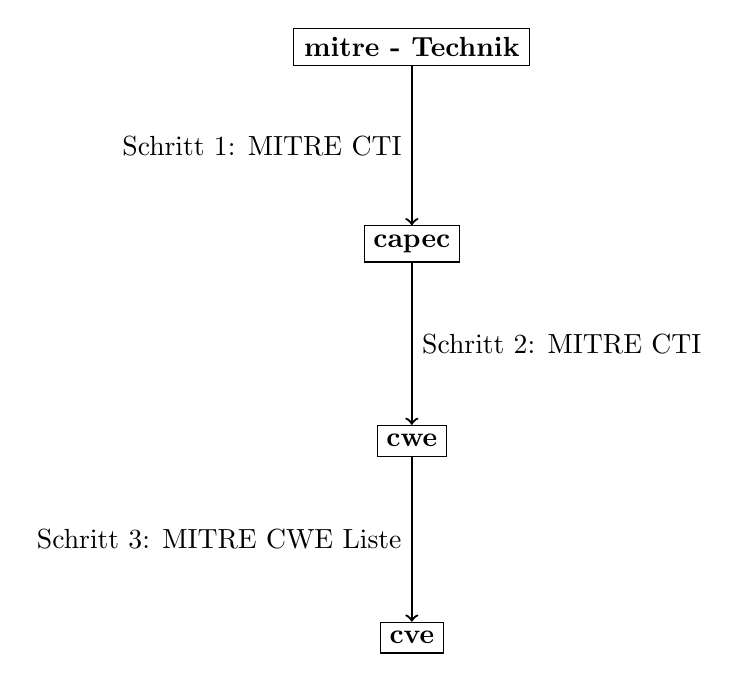
\begin{tikzpicture}[node distance=2cm, auto]
        % Nodes
        \node [rectangle, draw, text centered, minimum width=3cm] (mitre) {\textbf{\gls{mitre} - Technik}};
        \node [rectangle, draw, below of=mitre, yshift=-0.5cm] (capec) {\textbf{\gls{capec}}};
        \node [rectangle, draw, below of=capec, yshift=-0.5cm] (cwe) {\textbf{\gls{cwe}}};
        \node [rectangle, draw, below of=cwe, yshift=-0.5cm] (cve) {\textbf{\gls{cve}}};
        % Arrows
        \draw[->, thick] (mitre) -- (capec) node[midway, left] {Schritt 1: MITRE CTI};
        \draw[->, thick] (capec) -- (cwe) node[midway, right] {Schritt 2: MITRE CTI};
        \draw[->, thick] (cwe) -- (cve) node[midway, left] {Schritt 3: MITRE CWE Liste};
    \end{tikzpicture}
    \caption{Ablauf des Mappings von MITRE-Technik zu spezifischen CVE-Datum über die Kategorisierungssysteme MITRE, CAPEC, CWE und CVE.}
    \label{fig:mitre_mapping}
\end{figure}

Die spezifischen Angriffe, die im Dashboard angezeigt werden, stammen aus dem \gls{foran} \gls{at}. \todo{Relevanz??}

\par Das \gls{at} implementiert aktuell circa 250 Szenarien die Angriffsspuren erzeugen. Diese werden in 38 Techniken\footnote{Wenn ohne Zusatz von einer Technik gesprochen wird, meint das im Rahmen dieser Arbeit eine Technik aus einer der drei in Kapitel \ref{sec:datenquellen} definierten Matrizen. Nur wenn ausdrücklich von einer \gls{mitre}-Technik oder \gls{mitre}-Taktik gesprochen wird, meint dies Inhalte des \gls{attack}-Frameworks.} sortiert und übergeordnet auf 10 Taktiken verteilt. Eine Technik kann dabei in mehreren Taktiken angewendet werden.

\par Schritt 1 des in Abbildung \ref{fig:mitre_mapping} Ablaufs sucht für eine \gls{mitre}-Technik das zugehörige Angriffsmuster, den \gls{capec}. Die zugrundeliegenden Daten stammen aus dem von \gls{mitre} gepflegtem \gls{cti} Repository, in welchem die Daten regelmäßig aktualisiert im \textit{\gls{stix} 2.0}-Format veröffentlicht werden \autocite{IntroductionSTIX,MitreCtiCyber}. Die durch \gls{acema} gefundenen \glspl{capec} zu den \gls{mitre}-Techniken sind jedoch nicht vollständig, eine Erklärung und eine Lösung dafür wird in Kapitel \ref{sec:impl-anwendungVonAcema} präsentiert. Schritt 2 nutzt dasselbe Repository, denn dort sind für das jeweilige \gls{capec}-Objekt auch zugehörige \glspl{cwe} unter externen Referenzen verknüpft \autocite{CtiUSAGEmdMaster}. In Schritt 3 wird über das Pythonmodul \textit{cwe2} nach zugehörigen \glspl{cve} gesucht. Die zugrundeliegenden Daten für diese Abfrage stammen aus der \gls{cwe} Liste, die regelmäßig von \gls{mitre} veröffentlicht wird. Diese Liste enthält auch zugehörige \glspl{cve}, die in diesem Kontext \glqq{}beobachtete Beispiele\grqq{}\footnote{Auf Englisch: \glqq{}Observed Examples\grqq} genannt werden \autocite{AboutcodeorgCwe22024,CWEDownloads}. Um weitere Informationen wie \gls{cvss}, Angriffsvektoren und Veröffentlichungsdatum über einzelne \glspl{cve} zu beschaffen, wird die \gls{nvd} des \gls{nist} über die Python Module \verb|cve_lookup| und \verb|nvdlib| abgefragt \autocite{NVDLibNVDLibNIST,MachineThingCve_lookupLook,NVDHome}.
\par Die Besonderheit an \gls{acema} in Vergleich zu anderen \gls{mitre}-Technik zu \gls{cve}-Mappingtools ist, dass außerdem eine tiefgründige Analyse in the betroffenen O-RAN Bedrohungen aus dem Report der \gls{wg11} möglich ist. Dazu ist eine separate Zuordnung zwischen \gls{mitre}-Technik und O-RAN \textit{Threat-ID} aufzustellen.
\par Zusammenfassend müssen zwei Grundvoraussetzungen für die erfolgreiche Integration von \gls{acema} gegeben sein. Zum einen die Zuordnung einer oder mehrerer \gls{mitre}-Techniken zu einem Angriffsszenario des \gls{at}s. Zum zweiten die Zuordnung einer \gls{mitre}-Technik zu einer oder mehreren O-RAN \textit{Threat-IDs}.

\section{Grundprinzipien und Designentscheidungen für Visualisierungen}
\label{sec:auswahlDerVisualisierungstechniken}
Die Basis für die Wahl der Visualisierungstechniken im Dashboard wurden von Jonas Weber in seiner Arbeit gelegt \autocite{weberEvaluationDashboardTechniques}. \citeauthor{weberEvaluationDashboardTechniques} beschreibt darin grundlegende Prinzipien, die beim Design eines Dashboards eine wichtige Rolle spielen.
\par Das erste Prinzip beschreibt das Phänomen der präattentiven Wahrnehmung. Darunter versteht man die Wahrnehmung von visuellen Reizen, welches jedoch unterschwellig und ohne das Dazutuns von Aufmerksamkeit passiert. Man spricht auch von Vorbewusstsein \autocite{PraeattentiveWahrnehmung,mallotWahrnehmungPraeattentiveIm2021}. Über das Design von Dashboard auf Basis dieses neurologischen Konzepts gibt es zahlreiche wissenschaftliche Arbeiten, hervorgehoben sei dabei die Übersicht von \citeauthor{barrera-leonHowPreattentiveProcess2023} \autocite{barrera-leonHowPreattentiveProcess2023}. Anwendung findet dieses Prinzip in der Implementierung des Dashboards zum Beispiel beim Design der Zeitleiste. Im Listing \ref{fig:cvss-colors} ist dargestellt, wie der Schweregrad von Metriken eines \glspl{cve} anhand einer farblichen Kategorisierung eingeordnet wird. Die Farbwahl beschränkt sich hierbei auf vier deutlich voneinander unterscheidbaren Farben. Die Farbzuteilung ist in Tabelle \ref{tab:severity-color-mapping} dargestellt.
\begin{table}[H]
    \centering
    \caption{Farbzuordnung zu Schweregraden}
    \begin{tabular}{|c|c|}
        \hline
        \textbf{Farbe}                & \textbf{Schweregrad}  \\
        \hline
        \cellcolor[HTML]{6c757d} Grau & Keine Daten vorhanden \\
        \hline
        \cellcolor[HTML]{198754} Grün & Niedriger Schweregrad \\
        \hline
        \cellcolor[HTML]{ffc107} Gelb & Mittlerer Schweregrad \\
        \hline
        \cellcolor[HTML]{dc3545} Rot  & Hoher Schweregrad     \\
        \hline
    \end{tabular}
    \label{tab:severity-color-mapping}
\end{table}

Wissenschaftlich ist die kategorische Wahrnehmung von Farben unter anderem durch die wissenschaftliche Arbeit von \citeauthor{cliffordColorCategoriesAffect2010} bewiesen \autocite{cliffordColorCategoriesAffect2010}. Die technische Implementierung der Farbkategorisierung ist in Kapitel \ref{sec:impl-cvssIntegration} erläutert.
%
\begin{figure}[H]
    \centering
    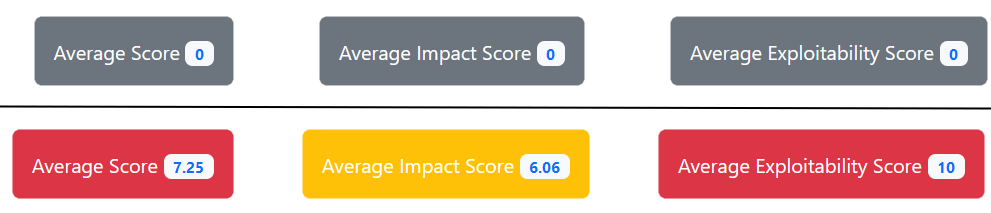
\includegraphics[width=0.8\textwidth]{cvss-colors}
    \caption{Farbkategorien zur Darstellung von Metriken}
    \label{fig:cvss-colors}
\end{figure}
%
\par Ein weiteres Prinzip, welches beim Visualisieren von Daten eine zentrale Bedeutung hat, wurde 1983 von \citeauthor{tufteBookReviewsVisual1984} als \textit{data-ink}-Prinzip definiert. Das Prinzip besagt, dass der Anteil der genutzten Farbe um die Daten darzustellen möglichst hoch sein soll. Damit soll die Darstellung von nicht-daten-bezogener Ausschmückung in der Visualisierung vermieden werden \autocite{tufteBookReviewsVisual1984}. An einem praktischen Beispiel kann jedoch gezeigt, dass ein geringeres \textit{data-ink} Verhältnis nötig sein kann, um Daten effizient darzustellen. In Kapitel \ref{sec:tech-foran} ist der Dateninhalt eines Artefaktes beschrieben. Als zentrale zu visualisierende Daten liegen jeweils das Start- und Enddatum der Artefakte vor. Die Abbildung \ref{fig:high-data-ink} zeigt die Darstellung von mehreren Artefakten auf einer Zeitleiste. Das \textit{data-ink} Verhältnis ist in dieser Darstellung sehr hoch, da tatsächlich nur die Start- und Endzeitpunkte dargestellt sind. Im Vergleich dazu wird in Abbildung \ref{fig:low-data-ink} die Zeitspanne zwischen den jeweiligen Daten eines Artefaktes zusätzlich farblich dargestellt. Es wird erkennbar, welche Punkte Start- oder Endpunkte sind. Dies war in Abbildung \ref{fig:high-data-ink} nicht intuitiv erkenntlich. Es ist in diesem Fall sinnvoll ein geringeres \textit{data-ink} Verhältnis zu erzielen, um Klarheit und Intuition zum Lesen zu schaffen. Die technische Konfiguration der Zeitleiste ist in Kapitel \ref{sec:impl-others} erläutert.
%
\begin{figure}[H]
    \centering
    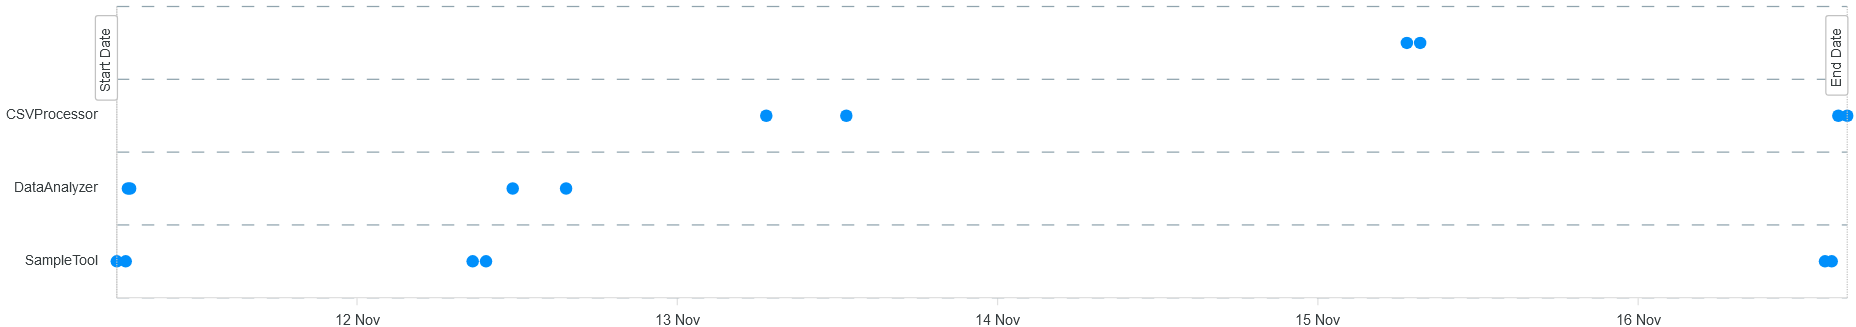
\includegraphics[width=1\textwidth]{high-data-ink}
    \caption{Hohes \textit{data-ink} Verhältnis}
    \label{fig:high-data-ink}
\end{figure}
%
\begin{figure}[H]
    \centering
    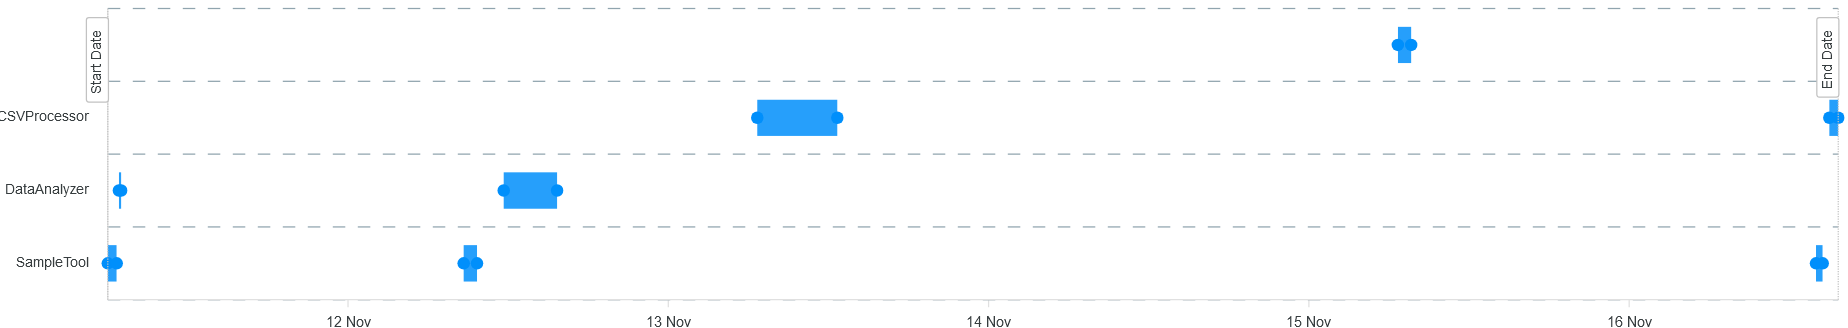
\includegraphics[width=1\textwidth]{low-data-ink}
    \caption{Niedriges \textit{data-ink} Verhältnis}
    \label{fig:low-data-ink}
\end{figure}
%
\par Diese beiden Prinzipien und andere Best Practices wurden auch bei Weiter- und Neuentwicklungen bei Visualisierung im Dashboard gewahrt. Bei der Darstellung des Angriffspfads und der Netzwerktopologie wurden bewusste design-technische Entscheidungen getroffen. Die Angriffspfads-Visualisierung enthält nicht viele Daten, nimmt aber einen großen Platz auf der Detailübersicht eines Artefaktes ein. Der Angriffsgraph und Netzwerkgraph sind beim Laden der Seite nicht direkt, sondern nur nach einem bewussten Scrollen sichtbar. So wird der Nutzer\footnote{In dieser Arbeit wird aus Gründen der besseren Lesbarkeit das generische Maskulinum für eine Person verwendet, die das Dashboard nutzt. Alle Geschlechteridentitäten werden dabei ausdrücklich mitgemeint.} nicht mit zu vielen Informationen auf einmal überladen. Die Graphen werden nicht als statische Bilder eingebettet. So lassen sich weitere Funktionen wie Tooltipps, dynamischer Zoom und die Verschiebbarkeit der einzelnen Elemente realisieren. Ein Tooltip hat hier die Funktion, zusätzliche hilfreiche Information zu liefern, wenn der Nutzer mit dem Mauszeiger auf ein Element zeigt \autocite{TooltipCarbonDesign}. Die Darstellung eines Tooltips ist in Abbildung \ref{fig:tooltip} gezeigt. Über die Verschiebbarkeit der Elemente kann das Diagramm angepasst werden, um es verständlicher darzustellen oder für einen Export vorzubereiten. Die Graphen können über gängige Browser per \textit{Rechtsklick, Speichern unter / In neuem Tab öffnen} als \verb|.png| Datei exportiert werden. Die technische Implementierung des Angriffsgraphen ist in Kapitel \ref{sec:impl-visualisierungDesAngriffspfads} erläutert.
%
\begin{figure}[H]
    \centering
    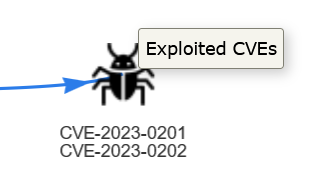
\includegraphics[width=0.5\textwidth]{tooltip}
    \caption{Tooltip auf einem Element im Angriffsgraphen}
    \label{fig:tooltip}
\end{figure}
%
\par Der Ablauf und das Ergebnis der Implementierung der Graphen sind in Kapitel \ref{sec:impl-visualisierungDesAngriffspfads} gezeigt.
\section{Werkzeuge und Technologien}
\label{sec:Entwicklungsumgebung}
In diesem Kapitel wird etwas tiefer auf die Tools eingegangen, die zur Umsetzung der Implementierung des Dashboards genutzt wurden. Informationen über die generelle Architektur, genutzte Programmiersprachen und Technologien finden sich in Kapitel \ref{sec:tech-dashboard}. Zu Beginn wurde die Entwicklung auf einer rein lokalen Umgebung durchgeführt. Über das von MongoDB zur Verfügung gestellte \gls{cli} lief ein MongoDB-Server, ein per \verb|go build| gebaute Dashboard-Server und der per \verb|yarn dev| gestartete Vite-Entwicklungs-Server auf dem lokalen Rechner \autocite{MongoDBDeveloperData,Vite}. Die Testdaten stammten aus dem Gitlab-Repo und sind von Jonas Weber zur Verfügung gestellt \autocite{AddExampleData2023}. Die Qualität und Menge der Testdaten waren für den Anfang ausreichend. Der Testdatensatz wurde seitdem aktualisiert, um den aktuellen Stand der Daten zu repräsentieren, und kann über die MongoDB \gls{cli} mit \verb|mongoimport| geladen werden \autocite{JSONMongoDB}. Um auf aktuellen Daten zu arbeiten und näher an der etablierten Testumgebung zu sein, wurde ab dem 7. August 2024 eine \gls{vm} in der \gls{dnlab}-Umgebung der TH Köln genutzt. Die Anwendung kann dann entweder weiterhin lokal auf der \gls{vm} oder zentralisiert per Ansible bereitgestellt werden \autocite{HomepageAnsibleCollaborative}. Ansible ist ein Tool zur Orchestrierung von Systemen und Software, welches durch die Ausführung von Skripten einen spezifischen technischen Zustand herstellt \autocite{ansiblecollaborativeetalHowAnsibleWorks2024}. Für die Ausführung des \gls{acema}-Quellcodes ist das Aufsetzen einer Python-Umgebung nötig \autocite{klement2023acema,WelcomePythonorg}.
Bei der Implementierung des Dashboards wurde für die Entwicklung und das Debugging gelegentlich ChatGPT-4 von OpenAI genutzt, um allgemeine Programmierfragen zu klären und Unterstützung bei Bearbeitung von repetitiven Aufgaben zu erhalten. 
\todo{Hab ich noch andere Tools genutzt??}